\chapter{Validation}
\section{Results}
\par The experiment was carried out across the first half of the Spring 2017 quarter at Cal Poly. 130 students signed up across 4 classes. By the end of the experiment, just over 3200 answers had been submitted to the application.

\subsection{Data Gathering}
\subsubsection{Final Survey}
\par After the experiment was concluded, all participants were sent a link to a survey where they could give feedback about their overall experience using \textit{Polycommit}. As an incentive, any participant who filled out the survey received +3 Commitment and +50 points (equal to an additional entry in the gift card raffle). A total of 70 participants filled out the post-experiment survey.

\subsubsection{Midterm Scores}
\par In order to gauge the effectiveness of \textit{Polycommit}, we collected scores on quizzes and exams and aggregated the data to be analyzed. For \textbf{Introduction to Operating Systems}, data collection was extremely simple as all the quizzes and midterms were administered through an online exam. This allowed us to easily obtain data on how students performed on specific midterm questions that aligned with questions asked in \textit{Polycommit}.

\par However, the other classes were not as simple. The other classes administered paper midterms, and we did not have access to the papers as they were being graded. As such, we administered a secondary survey to all the students in the class asking them to input their midterm scores for various questions.

\subsection{Limitations}
\par Certain restrictions were necessary in order to run this experiment. Most importantly, according to Cal Poly's human research regulations, studies about educational tools must be offered to all participants in a class. Thus, there was no true "control group" since any student could opt-in or opt-out of using the application.

\par As noted above, students were asked to input their midterm scores in an online form. We have no way of determining if this data was accurately entered; students may feel tempted to enter a higher score than they actually received.

\subsection{Overall Data}
\subsubsection{Cramming vs. Commitment}
\par First, consider the relationship between a student's overall score on the midterm and their Commitment (\textbf{\hyperref[fig:comm_vs_score]{Figure \ref*{fig:comm_vs_score}}}). No student that actively used the app (more than 10 Commitment) got less than 30/50 as a final score. This supports the idea that students benefit from consistent repetition over a longer period of time.
 
 \par 
 
 \begin{figure}[ht]
 	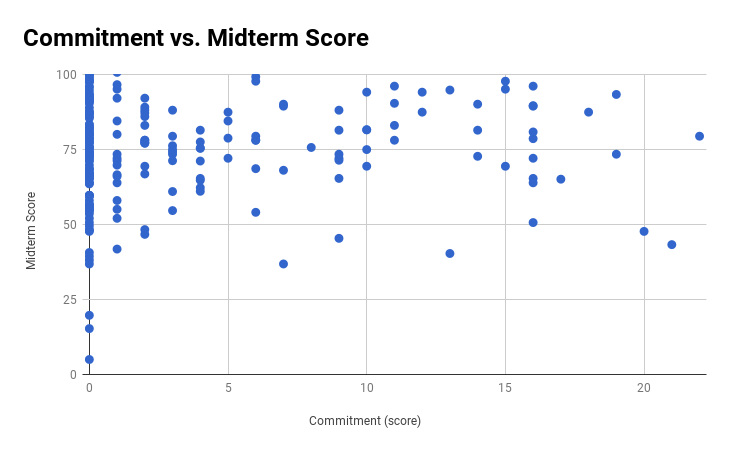
\includegraphics{figures/commitment-data1}
 	\caption{Graph of Commitment versus the student's score on the midterm for CPE 453.}
 	\label{fig:comm_vs_score}
 \end{figure}


\begin{figure}[ht]
	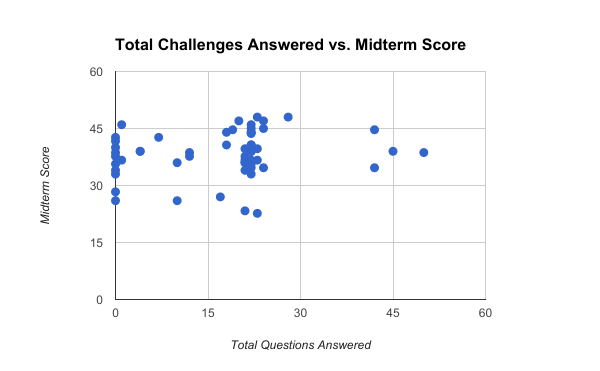
\includegraphics{figures/cramming-data}
	\caption{Graph of Total Questions Answered vs. the student's score on the midterm for CPE 453.}
	\label{fig:cramming}
\end{figure}
 
 \par Next, consider the mean of all midterm scores between students that didn't answer \textit{any} questions vs. the ones that did. Students that didn't answer any questions in the app scored slightly higher on average than the students that didn't.
  
 \begin{tabular}{ r c c }
  & Users & Non-users \\
%  \hline			90 m
 Midterm Average & 39.37 & 36.27 \\
 Population Size & 43 & 21
\end{tabular}

 \begin{figure}
	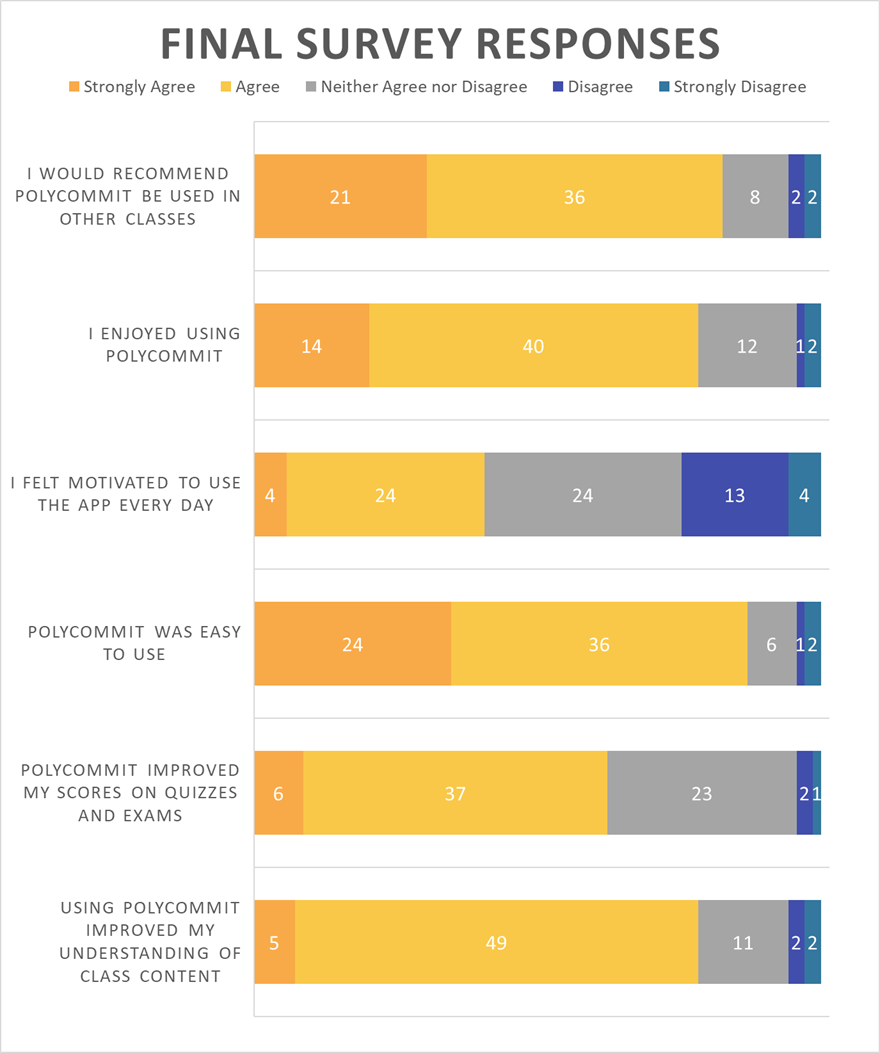
\includegraphics[width=1.0\linewidth]{figures/likert}
	\caption{Survey responses from users of Polycommit.}
	\label{fig:likert}
\end{figure}


\subsection{Individual Questions}
Certain questions on the midterm matched closely with the content of the questions that were repeated on \textit{Polycommit}. We can analyze midterm results to see if the students that drilled related problems in \textit{Polycommit} performed better on the related questions during the midterm.

\subsubsection{Introduction to Operating Systems}
One question that was shared between the midterm and \textit{Polycommit} was a question about the 4 conditions for deadlock. The question on the midterm asked students to choose the correct 4 conditions from a series of dropdowns, while the question on \textit{Polycommit} asked students to choose the \textit{incorrect} condition from the list. The 4 conditions for deadlock are:

\begin{enumerate}
	\item \textbf{Mutual exclusion}: At least one resource can only be
	held by one process at a time; this can result in other
	processes waiting for that resources
	\item \textbf{Hold and wait}: A process must be holding at least one
	resource while waiting for other resources (held by other
	processes)
	\item \textbf{No preemption}: Resources can only be released
	voluntarily by a process; Resources cannot be revoked
	\item \textbf{Circular wait}: A set of n waiting process $ {P_0, ..., P_n} $
	such that $ P_i $ is waiting for resources held by $ P_{(i+1)\%n} $
\end{enumerate}

\par The content of the question in \textit{Polycommit} and the question in the midterm are very similar. We can see if individuals who answered the Deadlock question correctly in \textit{Polycommit} had a higher score, on average, than the individuals who did not.

\begin{figure}[th!]
	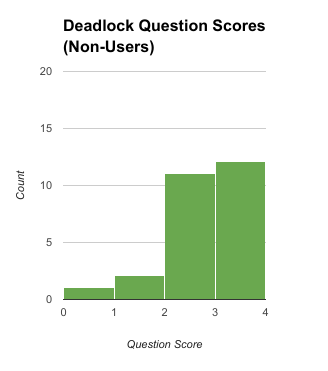
\includegraphics[width=0.5\linewidth]{figures/deadlock-nonusers}
	\caption{Count of scores for students that did \textit{not} make an attempt on the Deadlock question in \textit{Polycommit}.}
	\label{fig:deadlock-no}
\end{figure}

\begin{figure}[h!b]
	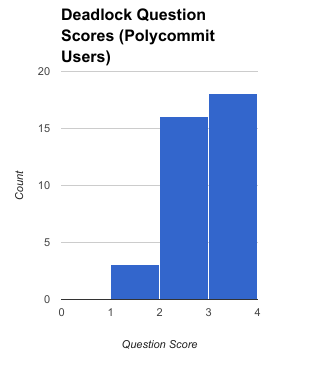
\includegraphics[width=0.5\linewidth]{figures/deadlock-users}
	\caption{Count of scores for students that \textit{did} make an attempt on the Deadlock question in \textit{Polycommit}.}
	\label{fig:deadlock-yes}
\end{figure}

\par The mean score for \textbf{non-users} is 3.30, and the mean score for \textbf{users} is 3.31. Thus, using \textit{Polycommit} had a negligible effect on the average score of the participants. However, note that 23/26 \textbf{non-users} received a score greater than 3, while 34/37 \textbf{users} received a score greater than 3. This could reflect the fact that \textit{Polycommit} only referenced 3 out of the 4 conditions for deadlock, as the 4th condition in the problem was a false plant. Although all 4 conditions are listed in the "explanation" field for the problem, by default if a student answers the question correctly they are brought back to the course page. Thus, students who participated in \textit{Polycommit} were only drilled on 3 out of the 4 conditions for deadlock, which would explain the overall performance on the midterm.

\par One interesting result comes by grouping midterm scores by the user's response to "Polycommit improved my scores on quizzes and exams" (See \textbf{\hyperref[fig:overconfidence]{Figure \ref*{fig:overconfidence}}}). Students who reported that Polycommit did \textit{not} improve their scores scored substantially higher than students who did. One explanation for this is that students who 

\begin{figure}[h]
	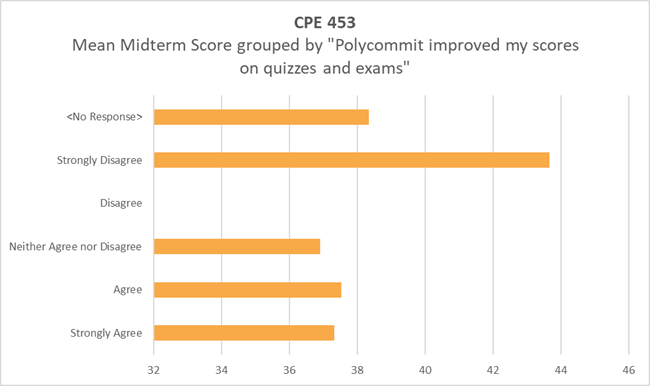
\includegraphics[width=1.0\linewidth]{figures/improved-vs-score}
	\caption{Mean midterm score grouped by response to final survey question "Polycommit improved my scores on quizzes and exams."}
	\label{fig:overconfidence}
\end{figure}



% TO DO: Put statistics for individual questions here. Note that deadlock wasn't improved by much, SJF actually got worse. Bring up possibility that students who sought out the app perhaps had less prior understanding of the course content or less consistent original study habits, leading to a selection bias that made them perform more poorly.

% Then, bring in statistics from the final survey where respondents said that they enjoyed using the app, and thought it improved their scores on quizzes and exams.
 